% some arguments why ERP:
% - see Cohen 2014 muscle twitches: In our final set of analyses,we examined the ERPs—the time-domain EMG onset-locked EEG potential. Thiswas done mainly to replicate previous findings concerning the relationship between the ERP and partial errors.
% - moving towards an applicable metric to detect things online, hence must be computationally inexpensive, therefore ERPs
% - use ERP section as exemplary for understanding results
%In haptically richer environments, processing gets more accurate and hence amplifies the error signal originating in or near anterior cingulate cortex (ACC). Moving fast and experiencing richer haptic feedback impact error processing

\subsection{Single trial regression ERSP: posterior cingulate}
% \subsection{Hand movement impacts error processing in independent anterior EEG sources}

\begin{figure}[h]
  \begin{flushleft}\textbf{A}\end{flushleft}
  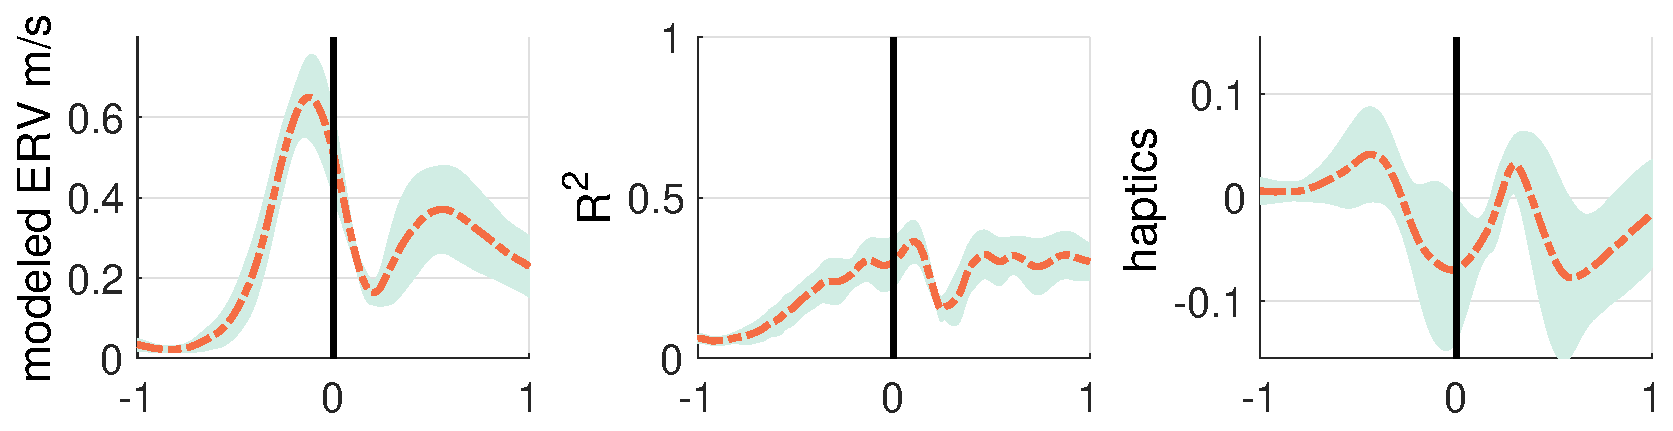
\includegraphics[width=\textwidth]{figures/vel_mocap_1.eps}
  \label{vel_erp_mismatch}
  \caption{Event-related velocity (ERV) succeeding premature collision.}
\end{figure}

\begin{figure}[h]
  \centering
  \caption{ERSP ACC}
\end{figure}
